
% !TEX root =../ECE343_Slides_Rogers.tex


%%%%%%%%%%%%%%%%%%%%%%%%%%%%%%%%%%%%%%%%%%%%%%%%%%%%%%
%%%%%%%%%%%%%%%%%%%%%%%%%%%%%%%%%%%%%%%%%%%%%%%%%%%%%%

\section{Schedule}

\begin{frame}{}
\renewcommand{\arraystretch}{1}
	\begin{textblock}{14}(0.5,1.75)
	\def\myfontsize{footnotesize}
	\setcounter{mylnum}{24}
%\def\myfontsize{normalsize}
\begin{center}
\begin{\myfontsize}
\begin{tabular}{| c | l | c | l |}
\hline
\textbf{Lesson} 		  	& \textbf{Topics}             & \pbox{5cm}{\textbf{Reading}}	& \textbf{Notes}		\\ \hline\hline
\ifnum\lessonNum=\value{mylnum} \rowcolor{green!20!white}\fi
	\themylnum  
	& BVP (Capacitor, Coax), Electric Potential	
	& 5.16
	&  LO 5.3  
\stepcounter{mylnum}\\ \hline \hline
\ifnum\lessonNum=\value{mylnum} \rowcolor{green!20!white}\fi
	\themylnum 	
	& Electric Boundary Conditions
	& 5.18-5.22	
	& LO 5.4			
\stepcounter{mylnum}\\ \hline
\ifnum\lessonNum=\value{mylnum} \rowcolor{green!20!white}\fi
	\themylnum 	
	& BC's/Capacitance			
	& 5.23-5.24
	& 	
\stepcounter{mylnum}\\ \hline
\ifnum\lessonNum=\value{mylnum} \rowcolor{green!20!white}\fi
	\themylnum 	
	& Electrostatic Lab			
	& Lab packet
	& 	
\stepcounter{mylnum}\\ \hline
\rowcolor{gray!20!white}\multicolumn{4}{| c |}{\textbf{Chapter 6: Steady Current \& Conductivity}}	\\ \hline\hline
\ifnum\lessonNum=\value{mylnum} \rowcolor{green!20!white}\fi
	\themylnum 	
	& Current density, Conductivity, Resistance
	& Ch. 6
	&   					
\stepcounter{mylnum}\\ \hline\hline
\rowcolor{gray!20!white}\multicolumn{4}{| c |}{\textbf{Chapter 7: Magnetostatics}}						\\ \hline\hline
\ifnum\lessonNum=\value{mylnum} \rowcolor{green!20!white}\fi
	\themylnum 	
	&  Magnetic Fields, Gauss' Law for Magnetism	
	& 7.1-7.3		
	&LO 7.1-7.2 \textbf{GR 2} 				
\stepcounter{mylnum}\\ \hline
\ifnum\lessonNum=\value{mylnum} \rowcolor{green!20!white}\fi
	\themylnum 	
	& Ampere's Law 	
	& 7.4-7.5, 7.9
	& LO 7.3		
\stepcounter{mylnum}\\ \hline 
\ifnum\lessonNum=\value{mylnum} \rowcolor{green!20!white}\fi
	\themylnum 	
	&  Ampere's Law Applied
	&  7.6-7.8
	& LO 7.3
\stepcounter{mylnum}\\ \hline 
\ifnum\lessonNum=\value{mylnum} \rowcolor{green!20!white}\fi
	\themylnum	
	& Magnetic Boundary Conditions	
	& 7.10-7.14	
	& LO 7.4 		
\stepcounter{mylnum}\\ \hline 
\ifnum\lessonNum=\value{mylnum} \rowcolor{green!20!white}\fi
	\themylnum  
	& Magnetostatics Lab
	& Lab packet
	&  		
\stepcounter{mylnum}\\ \hline \hline
\rowcolor{gray!20!white}\multicolumn{4}{| c |}{\textbf{Chapter 8: Time-Varying Fields}}					\\ \hline\hline
\ifnum\lessonNum=\value{mylnum} \rowcolor{green!20!white}\fi
	\themylnum 	
	& Faraday's Law, Displacement Current, Maxwell Eqns
	& 8.3, 8.8, 8.9
	& LO 8.1
\stepcounter{mylnum}\\ \hline 
\ifnum\lessonNum=\value{mylnum} \rowcolor{green!20!white}\fi
	\themylnum	
	& Faraday's Law, Displacement Current, Maxwell Eqns 
	&  8.3, 8.8, 8.9
	& LO 8.2-8.3
\stepcounter{mylnum}\\ \hline 

\rowcolor{gray!20!white}\multicolumn{4}{| c |}{\textbf{Chapter 9: Plane Waves in Lossless Media}}					\\ \hline\hline
\ifnum\lessonNum=\value{mylnum} \rowcolor{green!20!white}\fi
	\themylnum	
	& Maxwell's Equations in lossless, source-free region		
	& 9.1-9.2
	& LO 9.1	 
\stepcounter{mylnum}\\ \hline
\ifnum\lessonNum=\value{mylnum} \rowcolor{green!20!white}\fi
	\themylnum	
	& Maxwell's Equations in lossless, source-free region		
	& 9.1-9.2
	& LO 9.1	 
\stepcounter{mylnum}\\ \hline
%\ifnum\lessonNum=\value{mylnum} \rowcolor{green!20!white}\fi
%	\themylnum	
%	& Flex day
%	& 
%	& \textbf{GR 3}			 					
%\stepcounter{mylnum}\\ \hline 
\ifnum\lessonNum=\value{mylnum} \rowcolor{green!20!white}\fi
	\themylnum	
	& Uniform Plane Waves \& Polarization
	& 9.4-9.6
	& LO 9.2-9.3			
\stepcounter{mylnum}\\ \hline 
\ifnum\lessonNum=\value{mylnum} \rowcolor{green!20!white}\fi
	\themylnum	
	& Normal Incidence
	& Vol 2, 5.6-5.7
	&  LO 9.4-9.5
\stepcounter{mylnum}\\ \hline 
\ifnum\lessonNum=\value{mylnum} \rowcolor{green!20!white}\fi
	\themylnum	
	& Oblique Incidence			
	& Vol 2, 5.6-5.7
	& LO 9.5
\stepcounter{mylnum}\\ \hline 
\ifnum\lessonNum=\value{mylnum} \rowcolor{green!20!white}\fi
	\themylnum	
	& Oblique Incidence			
	& Vol 2, 5.6-5.7
	& LO 9.5
\stepcounter{mylnum}\\ \hline 
\ifnum\lessonNum=\value{mylnum} \rowcolor{green!20!white}\fi
	\themylnum	
	& Incidence Lab			
	& TBD
	& LO 9.5
\stepcounter{mylnum}\\ \hline 
%\ifnum\lessonNum=\value{mylnum} \rowcolor{green!20!white}\fi
%	\themylnum	
%	& Wrapup
%	& 
%	& 		 					
%\stepcounter{mylnum}\\ \hline 

\end{tabular}			
\end{\myfontsize}
\end{center}

	\end{textblock}
\end{frame}

%%%%%%%%%%%%%%%%%%%%%%%%%%%%%%%%%%%%%%%%%%%%%%%%%%%%%
%%%%%%%%%%%%%%%%%%%%%%%%%%%%%%%%%%%%%%%%%%%%%%%%%%%%%

\def\obja{ I can apply Coloumb's Law to use direct integration to calculate the electric field due to charge density in varoius geometries, including rectangular, cylindrical, and spherical coordinate systems. }
\def\objb{ I can apply the integral and differential forms of Gauss' Law to calculate the electric field due to charge density in various geometries, including rectangular, cylindrical, and spherical coordinate systems. }
\def\objc{ I can calculate the electric field from the scalar electric potential in a variety of geometries.}
\def\objd{ I can apply the electric field boundary conditions to calculate electric fields on both sides of a material boundary. }
\begin{frame}{Ch 5 Learning Objectives}
	\begin{textblock}{14}(0.5,2.5)
	\begin{myblock}[0.95]{}
	\begin{small}
	\begin{enumerate}[{5}.1]
		\ifnum\objNum=1
			\item \alert{ \obja }
		\else 
			\item \obja
		\fi 
		\ifnum\objNum=2
			\item \alert{ \objb }
		\else 
			\item \objb
		\fi 
		\ifnum\objNum=3
			\item \alert{ \objc }
		\else 
			\item \objc
		\fi 
		\ifnum\objNum=4
			\item \alert{ \objd }
		\else 
			\item \objd
		\fi 	
	\end{enumerate}
	\end{small}
	\end{myblock}
	\end{textblock}
\end{frame}

%%%%%%%%%%%%%%%%%%%%%%%%%%%%%%%%%%%%%%%%%%%%%%%%%%%%%%%
%%%%%%%%%%%%%%%%%%%%%%%%%%%%%%%%%%%%%%%%%%%%%%%%%%%%%%%
%
%\begin{frame}{1D Boundary Value Problem}
%
%\begin{textblock}{6}(0.5,3)
%\begin{center}
%\begin{circuitikz}[scale=1]
%	\draw (0,0) to[battery,a_=\myv{0}] ++(0,3)
%					to[short] ++(3,0)
%					to[short] ++(0,-0.75)
%					to[open] ++(0,-1.5)
%					to[short] ++(0,-0.75)
%					to[short] ++(-3,0);
%	\node[ground] at (1.5,0){};
%	% draw the capacitor
%	\fill[pattern=north west lines, pattern color=gray!50!white] (1.25,0.75) rectangle (4.75,2.25);
%	\draw[thick] (1.25,2.25) -- (4.75,2.25) node[right] {$z=d$}; % top wall
%	\draw[thick] (1.25,0.75) -- (4.75,0.75) node[right] {$z=0$}; % bottom
%	\foreach \x in {2,2.15,...,4}
%	{
%		\node at (\x,2.5){\tiny +};
%		\node at (\x,0.5){\tiny -};
%	}
%\end{circuitikz}
%\end{center}
%
%\alert{
%\eq{
%	V &= \dfrac{\myv{s}}{d} z \\
%	\vec{E} &=  -\nabla V = -\zhat\partd{}{z} \lp \dfrac{\myv{s}}{d} z \rp = -\zhat\dfrac{\myv{s}}{d}
%} % end eq
%} % end alert
%
%\end{textblock}
%
%\end{frame}


%%%%%%%%%%%%%%%%%%%%%%%%%%%%%%%%%%%%%%%%%%%%%%%%%%%%%%%%%%%%%%%
%%%%%%%%%%%%%%%%%%%%%%%%%%%%%%%%%%%%%%%%%%%%%%%%%%%%%%%%%%%%%%%

\section{Electric Field Boundary Conditions}
\begin{frame}{Static Electric Fields with Boundary}
\begin{textblock}{14.5}(0.5,4)
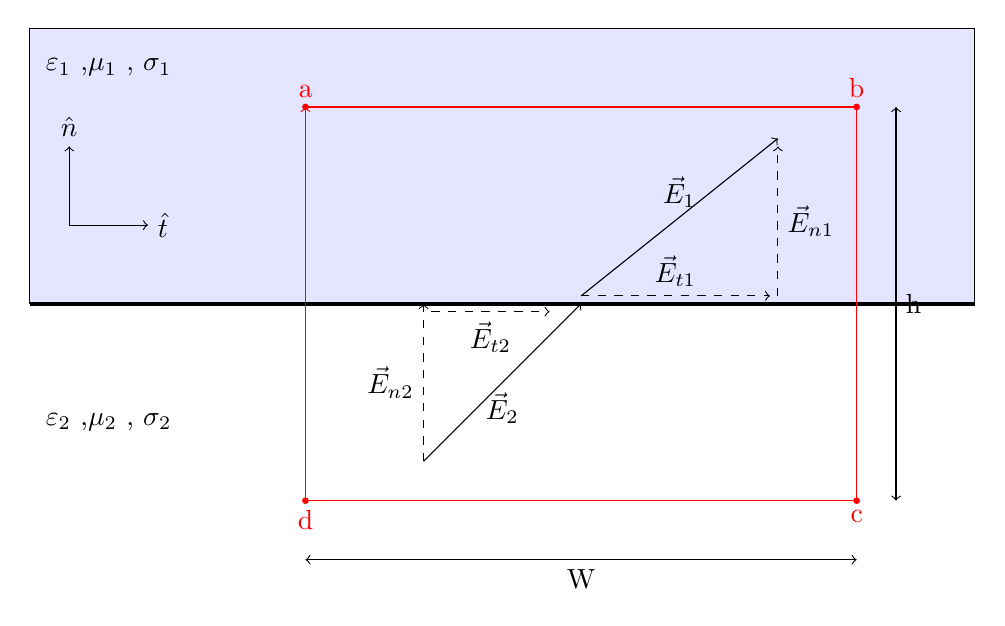
\begin{tikzpicture}

	\draw[fill=blue!10!white] (0,0) rectangle (12,3.5);
	\draw[ultra thick, black] (0,0) --++ (12,0);
	\node at (1,3) {$\varepsilon_1$ ,$\mu_1$ , $\sigma_1 $};
	\node at (1,-1.5) {$\varepsilon_2$ ,$\mu_2$ , $\sigma_2 $};
	
	\draw[->] (0.5,1) --++ (1,0) node[right] {$\hat{t}$};
	\draw[->] (0.5,1) --++ (0,1) node[above] {$\hat{n}$};
	
	% material 2
	\draw[->] (5,-2) --++ (2,2) node[midway, below] {$\vec{E}_2$}; 
	\draw[->, dashed] (5,-2) --++ (0,2) node[left, midway] {$\vec{E}_{\text{n2}}$};
	\draw[->, dashed] (5.1,-0.1) --++ (1.5,0) node[below, midway] {$\vec{E}_{\text{t2}}$};
	
	% material 1
	\draw[->] (7, 0.1)  --++ (2.5,2) node[midway, above] {$\vec{E}_{1}$};
	\draw[->, dashed] (9.5, 0.1) --++ (0,1.9) node[right, midway] {$\vec{E}_{\text{n1}}$};
	\draw[->, dashed] (7,0.1) --++ (2.4,0) node[above, midway] {$\vec{E}_{\text{t1}}$};
	
	%contours
	\coordinate (a) at (3.5, 2.5);
	\coordinate (b) at (10.5, 2.5);
	\coordinate (c) at (10.5, -2.5);
	\coordinate (d) at (3.5, -2.5);	
	
	\draw[red, fill=red] (a) circle (1pt) node[above]  {a};
	\draw[red, fill=red] (b) circle (1pt) node[above]  {b};
	\draw[red, fill=red] (c) circle (1pt) node[below] {c};
	\draw[red, fill=red] (d) circle (1pt) node[below] {d};
	
	\path[draw=red, ->] (a) -| (b) -| (c) -| (d) -| (a);
	\draw[<->] (3.5,-3.25) --++ (7,0) node[midway, below] {W};
	\draw[<->] (11,2.5) --++(0,-5) node[midway, right] {h};
	%\draw[red, thick,->] (3.5,2.5) node[above left] {a} --++ (7,0) node[above right] {b} --++ (0,-5) node[below right] {c} --++ (-7,0) node[below left] {d} --++ (0,5);
\end{tikzpicture}

\end{textblock}
\end{frame}


%%%%%%%%%%%%%%%%%%%%%%%%%%%%%%%%%%%%%%%%%%%%%%%%%%%%%%%%%%%%%%%
%%%%%%%%%%%%%%%%%%%%%%%%%%%%%%%%%%%%%%%%%%%%%%%%%%%%%%%%%%%%%%%
\begin{frame}{Boundary Conditions: Transverse}
\begin{textblock}{14.5}(0.5,2)
\only<0|handout:1>{
\alert{
\eq{
	&\oint \myvec{E}\mycdot \vec{d\ell} = 0 \\ 
	&\int\myvec{E}\mycdot \vec{d\ell_{ab}} +  	\int\myvec{E}\mycdot \vec{d\ell_{bc}} + 	\int\myvec{E}\mycdot \vec{d\ell_{cd}} + 	\int\myvec{E}\mycdot \vec{d\ell_{da}} = 0 \\
	&\int\myvec{E}\mycdot \vec{d\ell_{ab}} = \int_a^b \myvec{E}_{\text{t1}}\mycdot \hat{t} d\ell = E_{\text{t1}} W\\
	&\int\myvec{E}\mycdot \vec{d\ell_{bc}} = \int_{b-h/2}^b \myvec{E}_{1}\mycdot \lp-\hat{n} \rp d\ell + 
	\int_{b-h/2}^c \myvec{E}_{2}\mycdot \lp-\hat{n} \rp d\ell =-\lp E_{\text{n1}} + E_{\text{n2}} \rp\dfrac{h}{2}  \\
	&\int\myvec{E}\mycdot \vec{d\ell_{cd}} = \int_c^d \myvec{E}_{\text{t2}}\mycdot \lp -\hat{t}\rp d\ell = -E_{\text{t2}} W\\
	&\int\myvec{E}\mycdot \vec{d\ell_{da}} = \int_d^{d+h/2} \myvec{E}_{2}\mycdot \lp \hat{n} \rp d\ell +
	\int_{d+h/2}^a \myvec{E}_{1}\mycdot \lp \hat{n} \rp d\ell = \lp E_{\text{n1}} + E_{\text{n2}} \rp\dfrac{h}{2}  \\
	&\implies \oint \myvec{E}\mycdot \vec{d\ell} =  E_{\text{t1}} W + -\lp E_{\text{n1}} + E_{\text{n2}} \rp\dfrac{h}{2} -E_{\text{t2}} W +  \lp E_{\text{n1}} + E_{\text{n2}} \rp\dfrac{h}{2} = 0 
} % end eq
}% end alert
} % end only
\end{textblock}
\end{frame}

%%%%%%%%%%%%%%%%%%%%%%%%%%%%%%%%%%%%%%%%%%%%%%%%%%%%%%%%%%%%%%%
%%%%%%%%%%%%%%%%%%%%%%%%%%%%%%%%%%%%%%%%%%%%%%%%%%%%%%%%%%%%%%%
\begin{frame}{Boundary Conditions: Transverse}
\begin{textblock}{14.5}(0.5,4)
\begin{myblock}[0.9]{Transverse}
\alert{
\eq{
	E_{\text{t1}} = E_{\text{t2}} \qquad \text{ or } \qquad \hat{n}_{21} \times \lp \vec{E}_{1} - \vec{E}_2 \rp = 0 
} % end eq
}% end alert
\end{myblock}
\end{textblock}
\end{frame}

%%%%%%%%%%%%%%%%%%%%%%%%%%%%%%%%%%%%%%%%%%%%%%%%%%%%%%%%%%%%%%%
%%%%%%%%%%%%%%%%%%%%%%%%%%%%%%%%%%%%%%%%%%%%%%%%%%%%%%%%%%%%%%%

\begin{frame}{Boundary Conditions: Normal}
\begin{textblock}{14.5}(0.5,3.5)
\begin{tikzpicture}

	\draw[fill=blue!10!white] (0,0) rectangle (12,3.5);
	\draw[ultra thick, black] (0,0) --++ (12,0);
	\node at (1,3) {$\varepsilon_1$ ,$\mu_1$ , $\sigma_1 $};
	\node at (1,-1.5) {$\varepsilon_2$ ,$\mu_2$ , $\sigma_2 $};
	
	\draw[->] (0.5,1) --++ (1,0) node[right] {$\hat{t}$};
	\draw[->] (0.5,1) --++ (0,1) node[above] {$\hat{n}$};
	
	% material 2
	\draw[->] (5,-2) --++ (2,2) node[midway, below] {$\vec{E}_2$}; 
	\draw[->, dashed] (5,-2) --++ (0,2) node[left, midway] {$\vec{E}_{\text{n2}}$};
	\draw[->, dashed] (5.1,-0.1) --++ (1.5,0) node[below, midway] {$\vec{E}_{\text{t2}}$};
	
	% material 1
	\draw[->] (7, 0.1)  --++ (2.5,2) node[midway, above] {$\vec{E}_{1}$};
	\draw[->, dashed] (9.5, 0.1) --++ (0,1.9) node[right, midway] {$\vec{E}_{\text{n1}}$};
	\draw[->, dashed] (7,0.1) --++ (2.4,0) node[above, midway] {$\vec{E}_{\text{t1}}$};
	\foreach\x in {0.5,1,1.5,...,11}{
		\node[red] at (\x,0.1) {+};
	}	
	
	\node[cylinder, shape border rotate=90, draw, minimum height=5cm, minimum width=7cm, red] at (7,0) {};
	
\end{tikzpicture}

\vspace{-16pt}
\only<0|handout:1>{
\alert{
\eq{
	\implies \oiint \vec{D} \mycdot \vec{dS} &= \rho_S
} % end eq
} % end alert
}
\end{textblock}
\end{frame}

%%%%%%%%%%%%%%%%%%%%%%%%%%%%%%%%%%%%%%%%%%%%%%%%%%%%%%%%%%%%%%%
%%%%%%%%%%%%%%%%%%%%%%%%%%%%%%%%%%%%%%%%%%%%%%%%%%%%%%%%%%%%%%%
\begin{frame}{Boundary Conditions: Normal}
\begin{textblock}{14.5}(0.5,3)
\only<0|handout:1>{
\alert{
\eq{
	&\text{Top } \longrightarrow \oiint \vec{D}\mycdot \vec{dS}_{\text{top}} = \oiint \vec{D}\mycdot \hat{n} dS = D_{\text{n1}} (\text{area}) \\
	&\text{Bottom } \longrightarrow \oiint \vec{D}\mycdot \vec{dS}_{\text{bottom}} = \oiint \vec{D}\mycdot \lp -\hat{n}\rp dS = -D_{\text{n2}} (\text{area}) \\
	&\text{Sides } \overset{h\rightarrow 0}{\longrightarrow} \oiint\vec{D}\mycdot\vec{dS}_{\text{sides}} = 0 
	&Q_{\text{enclosed}} \longrightarrow \iint \rho_S dS = \rho_S (\text{area}) \\
	&\implies D_{\text{n1}} - D_{\text{n2}} = \rho_S \qquad \text{or} \qquad \hat{n}_{21} \mycdot \lp \varepsilon_1 \vec{E}_1 - \varepsilon_2 \vec{E}_2 \rp = \rho_S
} % end eq
} % end alert
}
\end{textblock}
\end{frame}


%%%%%%%%%%%%%%%%%%%%%%%%%%%%%%%%%%%%%%%%%%%%%%%%%%%%%%%%%%%%%%%
%%%%%%%%%%%%%%%%%%%%%%%%%%%%%%%%%%%%%%%%%%%%%%%%%%%%%%%%%%%%%%%
\begin{frame}{Boundary Conditions: Summary}
\begin{textblock}{14.5}(0.5,4)
\begin{myblock}[0.9]{Electric Field Boundary Conditions}
\eq{
&\text{ Transverse: } \qquad \hat{n}_{21} \times \lp \vec{E}_1 - \vec{E}_2 \rp = 0 \\
&\text{ Normal: } \qquad \hat{n}_{21} \mycdot \lp \varepsilon_1 \vec{E}_1 - \varepsilon_2 \vec{E}_2 \rp = \rho_S
} % end eq
\end{myblock}
\end{textblock}
\end{frame}

%%%%%%%%%%%%%%%%%%%%%%%%%%%%%%%%%%%%%%%%%%%%
%%%%%%%%%%%%%%%%%%%%%%%%%%%%%%%%%%%%%%%%%%%%

\begin{frame}{Angle of Incidence}
\begin{textblock}{14.5}(0.5,4)
\begin{tikzpicture}

	\draw[fill=blue!10!white] (0,0) rectangle (12,3.5);
	\draw[ultra thick, black] (0,0) --++ (12,0);
	\node at (1,3) {$\varepsilon_1$ ,$\mu_1$ , $\sigma_1 $};
	\node at (1,-1.5) {$\varepsilon_2$ ,$\mu_2$ , $\sigma_2 $};
	
	\draw[->] (0.5,1) --++ (1,0) node[right] {$\hat{t}$};
	\draw[->] (0.5,1) --++ (0,1) node[above] {$\hat{n}$};
	
	% material 2
	\draw[->] (5,-2) --++ (2,2) node[midway, below] {$\vec{E}_2$}; 
	\draw[->, dashed] (5,-2) --++ (0,2) node[left, midway] {$\vec{E}_{\text{n2}}$};
	\draw[->, dashed] (5.1,-0.1) --++ (1.5,0) node[above, midway] {$\vec{E}_{\text{t2}}$};
	
	% material 1
	\draw[->] (7, 0.1)  --++ (2.5,2) node[midway, above] {$\vec{E}_{1}$};
	\draw[->, dashed] (9.5, 0.1) --++ (0,1.9) node[right, midway] {$\vec{E}_{\text{n1}}$};
	\draw[->, dashed] (7,0.1) --++ (2.4,0) node[below, midway] {$\vec{E}_{\text{t1}}$};
	
	% plane of incidence
	\draw[dashed, ultra thick, blue] (7,-2.5) --++ (0,5) node[above, blue] {Plane of Incidence}; 
	\draw[<-, red] (7.5,0.5) arc (45:110:0.5) node[midway, above] {$\theta_1$};
	\draw[<-, red] (6.5,-0.5) arc (225:290:0.5) node[midway, below] {$\theta_2$};
	\node[red, align=left] at (10,-2) {$\theta_1 = \text{tan}^{-1}\lp \dfrac{|E_{t1}|}{|E_{n1}|} \rp$ \\ $\theta_2 = \text{tan}^{-1}\lp \dfrac{|E_{t2}|}{|E_{n2}|} \rp$};
\end{tikzpicture}

\end{textblock}
\end{frame}

%%%%%%%%%%%%%%%%%%%%%%%%%%%%%%%%%%%%%%%%%%%%%%%%%%%%%%%%%%%%%%%
%%%%%%%%%%%%%%%%%%%%%%%%%%%%%%%%%%%%%%%%%%%%%%%%%%%%%%%%%%%%%%%
\begin{frame}{Boundary Conditions: Example}
\begin{textblock}{14.5}(0.5,3.5)
An electric field $\vec{E}_1$ is incident from free space onto a material with $\varepsilon_{2r} = 2$. If  $\vec{E}_2 = \xhat 3 + \yhat 4 + \zhat 5$, find $\vec{E}_1$ and the angle of incidence of each vector.

\vspace{12pt}

\scalebox{0.65}{
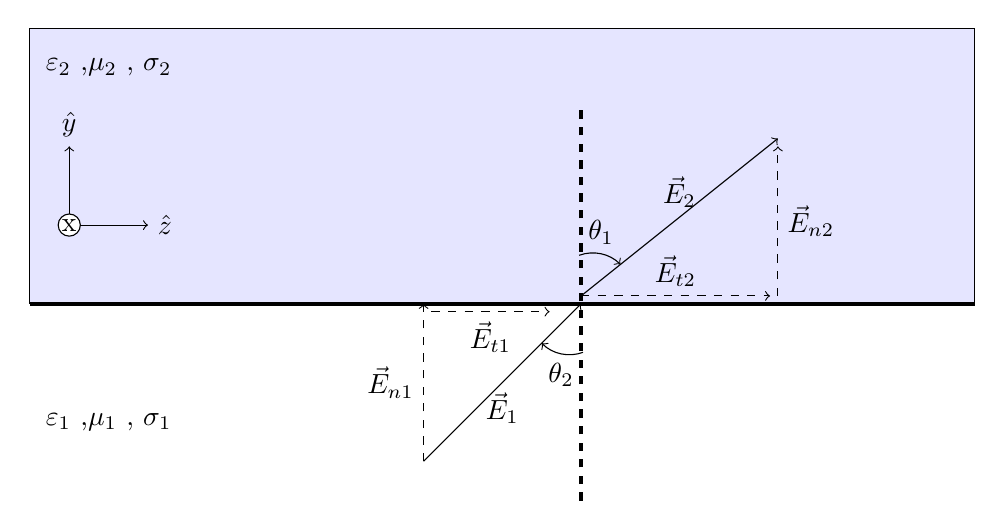
\begin{tikzpicture}

	\draw[fill=blue!10!white] (0,0) rectangle (12,3.5);
	\draw[ultra thick, black] (0,0) --++ (12,0);
	\node at (1,3) {$\varepsilon_2$ ,$\mu_2$ , $\sigma_2 $};
	\node at (1,-1.5) {$\varepsilon_1$ ,$\mu_1$ , $\sigma_1 $};
	
	\draw[->] (0.5,1) --++ (1,0) node[right] {$\hat{z}$};
	\draw[->] (0.5,1) --++ (0,1) node[above] {$\hat{y}$};
	\draw[black, fill=white] (0.5,1) circle (4pt) node {x};
	
	% material 1
	\draw[->] (5,-2) --++ (2,2) node[midway, below] {$\vec{E}_1$}; 
	\draw[->, dashed] (5,-2) --++ (0,2) node[left, midway] {$\vec{E}_{\text{n1}}$};
	\draw[->, dashed] (5.1,-0.1) --++ (1.5,0) node[below, midway] {$\vec{E}_{\text{t1}}$};
	
	% material 2
	\draw[->] (7, 0.1)  --++ (2.5,2) node[midway, above] {$\vec{E}_{2}$};
	\draw[->, dashed] (9.5, 0.1) --++ (0,1.9) node[right, midway] {$\vec{E}_{\text{n2}}$};
	\draw[->, dashed] (7,0.1) --++ (2.4,0) node[above, midway] {$\vec{E}_{\text{t2}}$};
	
	
	
	% plane of incidence
	\draw[dashed, ultra thick] (7,-2.5) --++ (0,5); 
	\draw[<-] (7.5,0.5) arc (45:110:0.5) node[midway, above] {$\theta_1$};
	\draw[<-] (6.5,-0.5) arc (225:290:0.5) node[midway, below] {$\theta_2$};
	
\end{tikzpicture}
} % end scalebox
\end{textblock}
\begin{textblock}{5}(10,6)
\alert{
\begin{small}
\eq{
	&\text{Transverse} \longrightarrow  \xhat, \zhat\\
	&\text{Normal} \longrightarrow \yhat \\
	} % end eq
\end{small}
	} % end alert
\end{textblock}
\end{frame}

%%%%%%%%%%%%%%%%%%%%%%%%%%%%%%%%%%%%%%%%%%%%%%%%%%%%%%%%%%%%%%%
%%%%%%%%%%%%%%%%%%%%%%%%%%%%%%%%%%%%%%%%%%%%%%%%%%%%%%%%%%%%%%%
\begin{frame}{Boundary Conditions: Example (cont'd)}
\begin{textblock}{8.5}(0.5,3)
\alert{
\begin{small}
\eq{
	&\circled{1} 
	\begin{cases}
		&\vec{E}_{\text{t2}} = \xhat 3 + \zhat 5 \implies | \vec{E}_{\text{t2}} | = \sqrt{3^2 + 5^2} = \sqrt{34}  \\
		&\vec{E}_{\text{n2}} = \yhat 4 \implies |\vec{E}_{\text{n2}}| = 4
	\end{cases} \\
	&\circled{2} \longrightarrow \theta_2 = \text{tan}^{-1} \lp \dfrac{| \vec{E}_{\text{t2}} | }{| \vec{E}_{\text{n2}} | } \rp =  \text{tan}^{-1} \lp \dfrac{\sqrt{34} }{4 } \rp = 55.6\mydeg \\
	&\circled{3} \longrightarrow \text{Normal BC}  \implies \hat{n}_{2,1} = -\yhat \\
	&\qquad -\yhat \mycdot \lp \varepsilon_1 \vec{E}_1 - \varepsilon_2 \vec{E}_2 \rp = 0  \\
	&\qquad -\yhat \mycdot \varepsilon_0 \vec{E}_1 + \yhat \mycdot \lb 2\varepsilon_0 \lp \xhat 3 + \yhat 4 + \zhat 5 \rp\rb = 0 \\
	&\qquad -\varepsilon_0 E_{1y} + 8\varepsilon_0 = 0 \\
	&\qquad \implies E_{1y}  = 8
} % end eq
\end{small}
} % end alert
\end{textblock}
\end{frame}

%%%%%%%%%%%%%%%%%%%%%%%%%%%%%%%%%%%%%%%%%%%%%%%%%%%%%%%%%%%%%%%
%%%%%%%%%%%%%%%%%%%%%%%%%%%%%%%%%%%%%%%%%%%%%%%%%%%%%%%%%%%%%%%
\begin{frame}{Boundary Conditions: Example (cont'd)}
\begin{textblock}{8.5}(0.5,3)
\alert{
\begin{small}
\eq{
	&\circled{4} \longrightarrow \text{Transverse BC}  \\
%	&\qquad \implies \vec{E}_{\text{t1}} = \vec{E}_{\text{t2}} \implies \vec{E}_{\text{t1} = \xhat 3 + \zhat 5 \\
	&\circled{5} \longrightarrow \vec{E}_1 = \xhat 3 + \yhat 8 + \zhat 5 \\
	&\circled{6} \longrightarrow \theta_1 = \text{tan}^{-1}\lp\dfrac{|\vec{E}_{\text{t1}}|}{|\vec{E}_{\text{n1}}|}\rp = \text{tan}^{-1}\lp \dfrac{\sqrt{34}}{8}\rp = 36\mydeg
} % end eq
\end{small}
} % end alert
\end{textblock}

\begin{textblock}{14.5}(0.5,7)
\begin{myblock}[0.9]{Summary}
\vspace{-12pt}
\alert{
\eq{
	\vec{E}_1 &= \xhat 3 + \yhat 8 + \zhat 5  \\
	\vec{E}_2 &= \xhat 3 + \yhat 4 + \zhat 5  \\
	\theta_1 &= 36\mydeg \\
	\theta_2 &= 55.6\mydeg
} % end eq
}% end alert
\vspace{-12pt}
\end{myblock}
\end{textblock}
\end{frame}
%%%%%%%%%%%%%%%%%%%%%%%%%%%%%%%%%%%%%%%%%%%%%%%%%%%%%%%%%%%%%%%
%%%%%%%%%%%%%%%%%%%%%%%%%%%%%%%%%%%%%%%%%%%%%%%%%%%%%%%%%%%%%%%
\begin{frame}{Your Turn: Example \#2}
\begin{textblock}{14.5}(0.5,3.5)
An electric field $\vec{E}_1$ is incident from free space onto a material with $\varepsilon_{2r} = 4$. If  $\vec{E}_2 = \xhat 3 + \yhat 4 + \zhat 5$, find $\vec{E}_1$ and the angle of incidence of each vector.

\vspace{12pt}

\scalebox{0.65}{
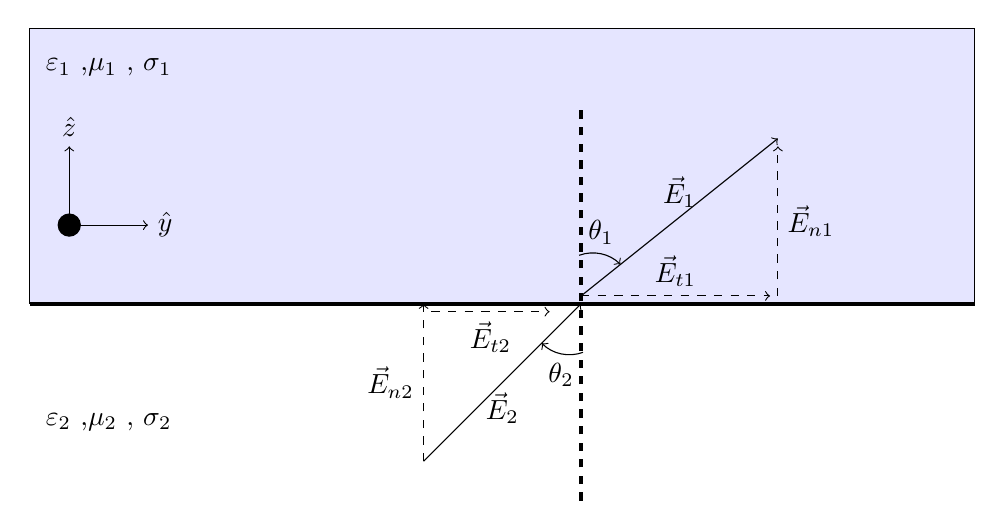
\begin{tikzpicture}

	\draw[fill=blue!10!white] (0,0) rectangle (12,3.5);
	\draw[ultra thick, black] (0,0) --++ (12,0);
	\node at (1,3) {$\varepsilon_1$ ,$\mu_1$ , $\sigma_1 $};
	\node at (1,-1.5) {$\varepsilon_2$ ,$\mu_2$ , $\sigma_2$};
	
	\draw[->] (0.5,1) --++ (1,0) node[right] {$\hat{y}$};
	\draw[->] (0.5,1) --++ (0,1) node[above] {$\hat{z}$};
	\draw[black, fill=black] (0.5,1) circle (4pt);
	
	% material 2
	\draw[->] (5,-2) --++ (2,2) node[midway, below] {$\vec{E}_2$}; 
	\draw[->, dashed] (5,-2) --++ (0,2) node[left, midway] {$\vec{E}_{\text{n2}}$};
	\draw[->, dashed] (5.1,-0.1) --++ (1.5,0) node[below, midway] {$\vec{E}_{\text{t2}}$};
	
	% material 1
	\draw[->] (7, 0.1)  --++ (2.5,2) node[midway, above] {$\vec{E}_{1}$};
	\draw[->, dashed] (9.5, 0.1) --++ (0,1.9) node[right, midway] {$\vec{E}_{\text{n1}}$};
	\draw[->, dashed] (7,0.1) --++ (2.4,0) node[above, midway] {$\vec{E}_{\text{t1}}$};
	
	
	
	% plane of incidence
	\draw[dashed, ultra thick] (7,-2.5) --++ (0,5); 
	\draw[<-] (7.5,0.5) arc (45:110:0.5) node[midway, above] {$\theta_1$};
	\draw[<-] (6.5,-0.5) arc (225:290:0.5) node[midway, below] {$\theta_2$};
	
\end{tikzpicture}
} % end scalebox
\end{textblock}
\begin{textblock}{5}(10,6)
\alert{
\begin{small}
\eq{
	&\text{Transverse} \longrightarrow  \\%\xhat, \yhat\\
	&\text{Normal} \longrightarrow \\%\zhat \\
	} % end eq
\end{small}
	} % end alert
\end{textblock}
\end{frame}

%%%%%%%%%%%%%%%%%%%%%%%%%%%%%%%%%%%%%%%%%%%%%%%%%%%%%%%%%%%%%%%
%%%%%%%%%%%%%%%%%%%%%%%%%%%%%%%%%%%%%%%%%%%%%%%%%%%%%%%%%%%%%%%
\begin{frame}{Your Turn: Example \#2}
\begin{textblock}{14.5}(0.5,4)

\end{textblock}
\end{frame}

%%%%%%%%%%%%%%%%%%%%%%%%%%%%%%%%%%%%%%%%%%%%%%%%%%%%%%%%%%%%%%%
%%%%%%%%%%%%%%%%%%%%%%%%%%%%%%%%%%%%%%%%%%%%%%%%%%%%%%%%%%%%%%%
\begin{frame}{Perfect Electric Conductors (PEC)}
\begin{textblock}{14.5}(0.5,2)
\begin{center}
\scalebox{0.75}{
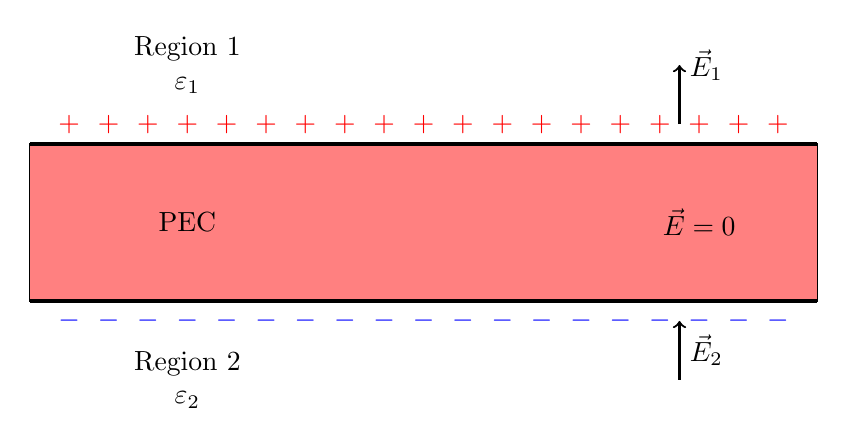
\begin{tikzpicture}
	\draw[fill=red!50!white] (0,0) rectangle ++(10,2); % PEC
	\draw[ultra thick] (0,0) --++(10,0); % lower PEC boundary
	\foreach \x in {0.5,1,...,9.5}{
		\node[blue] at (\x,-0.25) {$-$}; 
	} % lower boundary charges
	\draw[ultra thick] (0,2) --++(10,0); % upper PEC boundary
	\foreach \x in {0.5,1,...,9.5}{
		\node[red] at (\x,2.25) {$+$}; 
	} % upper boundary charges
	
	% material labels 
	\node[align=center] at (2,3) {Region 1 \\ $\varepsilon_1$};
	\node at (2,1) {PEC};
	\node[align=center] at (2,-1) {Region 2 \\ $\varepsilon_2$};
	
	% electric fields
	\draw[->, thick] (8.25,-1) --++ (0,0.75) node[midway, right] {$\vec{E}_2$};
	\node at (8.5,1) {$\vec{E} = 0$};
	\draw[->, thick] (8.25,2.25) --++ (0,0.75) node[right] {$\vec{E}_1$};
\end{tikzpicture}
} % end scalebox
\end{center}
\vspace{-26pt}
\begin{myblock}[0.9]{\small{Electric Field in a PEC}}
	\begin{small}
	\begin{enumerate}
		\item $\vec{E} = 0 $ inside a PEC 
		\item If $\vec{E}_{\text{PEC}} = 0$, then $\vec{E}_{\text{t,outside}} = \vec{E}_{\text{t,PEC}} = 0$
		\item Normal BC requires $\vec{E}_{\text{n, outside}} = \dfrac{\rho_S}{\varepsilon}$
		\item No static charge \textbf{inside} PEC  
	\end{enumerate}
	\end{small}
\end{myblock}


\end{textblock}
\end{frame}

%%%%%%%%%%%%%%%%%%%%%%%%%%%%%%%%%%%%%%%%%%%%%%%%%%%%%%%%%%%%%%%
%%%%%%%%%%%%%%%%%%%%%%%%%%%%%%%%%%%%%%%%%%%%%%%%%%%%%%%%%%%%%%%
\begin{frame}{Capacitance}
\begin{textblock}{14.5}(0.5,2.5)
\begin{myblock}[0.9]{Capacitance}
\begin{enumerate}
	\item Capacitance is the ability of a structure to store energy in an electric field $\longrightarrow C = \dfrac{Q}{V}$
	\item Depends on the geometry and permittivity of medium separating plates.
\end{enumerate}
\end{myblock}
\vspace{-12pt}
\only<0|handout:1>{
\begin{small}
\alert{
\eq{
	Q (t) & = \int_{t_0}^t I(\tau) d\tau + Q (t_0) \\
	\implies V (t) &= \dfrac{1}{C}\int_{t_0}^t I(\tau) d\tau + \dfrac{1}{C}Q (t_0) 					= \dfrac{1}{C}\int_{t_0}^t I(\tau) d\tau + V_0 \\
	\implies I(t) &= C\partd{}{t} V(t)
} % end eq
} % end alert
\end{small}
} % end handout
\end{textblock}
\end{frame}


%%%%%%%%%%%%%%%%%%%%%%%%%%%%%%%%%%%%%%%%%%%%%%%%%%%%%%%%%%%%%%%
%%%%%%%%%%%%%%%%%%%%%%%%%%%%%%%%%%%%%%%%%%%%%%%%%%%%%%%%%%%%%%%
\begin{frame}{Parallel Plate Capacitor}
\begin{textblock}{8}(0.5,2.5)
\begin{center}
\begin{circuitikz}[scale=1]
	% 
	\draw[->] (6,0.75) --++ (0.75,0) node[right] {$\rho$}; 
	\draw[->] (6,0.75) --++ (0,0.75) node[above] {$z$};
	\draw (0,0) to[battery,a^=\myv{0}, invert] ++(0,3)
					to[short] ++(3,0)
					to[short] ++(0,-0.75)
					to[open] ++(0,-1.5)
					to[short] ++(0,-0.75)
					to[short] ++(-3,0);
	\node[ground] at (1.5,0){};
	% draw the capacitor
	\fill[pattern=north west lines, pattern color=gray!50!white] (1.25,0.75) rectangle (4.75,2.25);
	\draw[thick] (1.25,2.25) -- (4.75,2.25) node[right] {$z=d$}; % top wall
	\draw[thick] (1.25,0.75) -- (4.75,0.75) node[right] {$z=0$}; % bottom
	\foreach \x in {2,2.15,...,4}
	{
		\node at (\x,2.5){\tiny +};
		\node at (\x,0.5){\tiny -};
	}
\end{circuitikz}
\end{center}
\vspace{-12pt}
\only<0|handout:1>{
\begin{small}
\alert{
\eq{
	V &= -\int_C \vec{E} \mycdot d\ell \\
	&= -\int_0^d \dfrac{1}{\varepsilon} \vec{D} \mycdot \lp \zhat dz \rp\\
	&= -\int_0^d \lp -\zhat \dfrac{\rho_s}{\varepsilon} \rp \mycdot \lp \zhat dz \rp \\
	V &= - \dfrac{\rho_S d}{\varepsilon} 
} % end eq
} % end alert
\end{small}
} % end handout
\end{textblock}

\begin{textblock}{8}(8.5,9.5)
	\only<0|handout:1>{
	\begin{small}
	\alert{
	Now the capacitance is:
	\eq{
		C &= \dfrac{Q}{V} = \dfrac{\rho_s A}{\frac{\rho_s d}{\varepsilon}} \\
		&= \dfrac{\varepsilon A}{d}
	} % end eq
	} % end alert
	\end{small}
	}% end handout
\end{textblock}
\end{frame}

%%%%%%%%%%%%%%%%%%%%%%%%%%%%%%%%%%%%%%%%%%%%%%%%%%%%%%%%%%%%%%%
%%%%%%%%%%%%%%%%%%%%%%%%%%%%%%%%%%%%%%%%%%%%%%%%%%%%%%%%%%%%%%%
\begin{frame}{Coaxial Capacitor }
\begin{textblock}{8}(0.5,4)
Find the capacitance for a coaxial capacitor of length (in $z$-dimension) $\ell$. 
\scalebox{1}{
\begin{circuitikz}
\draw[pattern=north west lines, pattern color=gray!50!white] (0,0) circle (1.5);
\draw[black,fill=white] (0,0) circle (0.5);
\fill[black] (0,0) circle (1pt); % origin
\draw (120:0) -- node[right]{$b$}(120:1.5);
\draw (200:0) -- node[above]{$a$}(200:0.5);
%\draw[dashed, -stealth] (90:0) -- (90:2);
% \draw[red,-stealth] (0,1.75) arc (90:120:1.5) node[above,red]{$\phi$};
\draw (0:0.5) to[short] ++(2,0)
			to[battery, , a^=\myv{0}] ++(0,-2)
			to[short] ++(-2.25,0)
			to[short] ++(0,0.5);
\end{circuitikz}
} % end scalebox
\only<0|handout:1>{
\alert{
\eq{
	\vec{E} &= \rhohat \dfrac{\rho_\ell}{2\pi\varepsilon \rho} \\
	Q &= \rho_{\ell} \ell
}
}
}
\end{textblock}

\begin{textblock}{8}(8.5,3)
\only<0|handout:1>{
\begin{small}
\alert{
\eq{
	V &= -\int_C \vec{E}\mycdot \vec{d\ell} \\
	&= -\int_{\rho=a}^b \lp \rhohat \dfrac{\rho_\ell}{2\pi\varepsilon \rho} \rp \mycdot \lp \rhohat d\rho \rp \\
	&= -\dfrac{\rho_\ell}{2\pi\varepsilon} \int_{\rho=a}^b \dfrac{1}{\rho}d\rho \\
	&= \dfrac{\rho_\ell}{2\pi\varepsilon}  \text{ln}\lp \dfrac{b}{a} \rp \\
	\implies C&= \dfrac{Q}{V} = \dfrac{\rho_\ell \ell}{\frac{\rho_\ell}{2\pi\varepsilon}  \text{ln}\lp \dfrac{b}{a} \rp  } \\
	&= \dfrac{2\pi\varepsilon\ell}{ \text{ln}\lp \dfrac{b}{a} \rp }
} % end eq
} % end alert
\end{small}
} % end handout 
\end{textblock}
\end{frame}


